\documentclass[oneside,12pt]{Classes/aesm_edspia}
\usepackage[utf8]{inputenc}
\usepackage[LFE,LAE,OT1]{fontenc}

\usepackage[french,english,arabic]{babel}

\pagestyle{fancy}

    \usepackage{graphicx}
 \begin{document}
\setlength{\parindent}{0pt}
\setlength{\topmargin}{0mm}
\setlength{\headheight}{0cm}
\setlength{\headsep}{0cm}
\setlength{\textheight}{20cm}
\setlength{\textwidth}{17cm}
\setlength{\marginparsep}{0cm}
\setlength{\marginparwidth}{0cm}
\setlength{\headheight}{0cm}
\setlength{\footskip}{0cm}

\pagestyle{fancy}


\begin{center}
\hbox{\raisebox{0.2em}{\vrule depth 0pt height 1pt width 17cm}}
\end{center}
\selectlanguage{arabic}
%\doublebox{
\begin{minipage}[c]{\textwidth}
  \textbf{خلاصة}\\ [0.4cm]
\footnotesize
يجب أن لا تتجاوز خمسة أسطر \\[0.4cm]
الكلمات الرئيسية:
    كلمة ١, كلمة ٢, كلمة ٣
\end{minipage}
%}
\\[1.5cm]
\begin{center}
\hbox{\raisebox{0.2em}{\vrule depth 0pt height 1pt width 17cm}}
\end{center}
\selectlanguage{french}
%\doublebox{
\begin{minipage}[c]{\textwidth}
\textbf{Résumé}\\[0.4cm]
\footnotesize
\textbf{Le résumé du rapport ne doit pas dépasser les cinq lignes.}
\\[0.4cm]
\textbf{Mots clés :} \textbf{Mot1, Mot2, Mot3...}
\end{minipage}
%}
\\[1.5cm]
\begin{center}
\hbox{\raisebox{0.2em}{\vrule depth 0pt height 1pt width 17cm}}
\end{center}
\selectlanguage{english}
%\doublebox{
\begin{minipage}[c]{\textwidth}
\textbf{Abstract}\\[0.4cm]
\footnotesize
\textbf{The abstract should not exceed five lines. }
\\[0.4cm]
\textbf{Keywords :} \textbf{Word1, Word2, Word3...}
\end{minipage}%}
\begin{center}
\begin{figure}
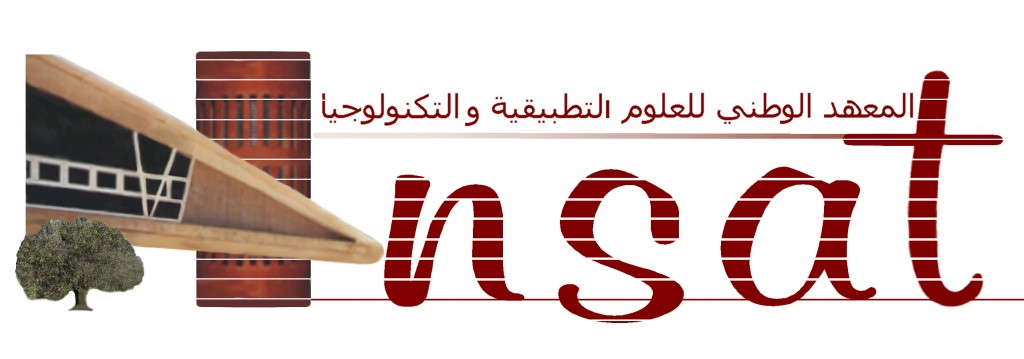
\includegraphics[scale=.1]{Cover/Figures/insat.jpg}
\end{figure}
\end{center}

\renewcommand{\footrulewidth}{1pt}
\fancyfoot[C]{\textbf{Institut National des Sciences Appliquées et de Technologie}}
\fancyfoot[L]{}
\fancyfoot[R]{}
\end{document}
